%; whizzy chapter
% -initex iniptex -latex platex -format platex -bibtex jbibtex -fmt fmt
% 以上 whizzytex を使用する場合の設定。


%     Tokyo Debian Meeting resources
%     Copyright (C) 2007 Junichi Uekawa

%     This program is free software; you can redistribute it and/or modify
%     it under the terms of the GNU General Public License as published by
%     the Free Software Foundation; either version 2 of the License, or
%     (at your option) any later version.

%     This program is distributed in the hope that it will be useful,
%     but WITHOUT ANY WARRANTY; without even the implied warranty of
%     MERCHANTABILITY or FITNESS FOR A PARTICULAR PURPOSE.  See the
%     GNU General Public License for more details.

%     You should have received a copy of the GNU General Public License
%     along with this program; if not, write to the Free Software
%     Foundation, Inc., 51 Franklin St, Fifth Floor, Boston, MA  02110-1301 USA

%  preview (shell-command (concat "xpdf " (replace-regexp-in-string "tex$" "pdf"(buffer-file-name)) "&"))
% 画像ファイルを処理するためにはebbを利用してboundingboxを作成。
%(shell-command "cd image200703; ebb *.png")

% real presentation (shell-command (concat "DISPLAY=:0.1 xpdf " (replace-regexp-in-string "tex$" "pdf"(buffer-file-name)) "&"))


%%ここからヘッダ開始。
\documentclass[mingoth,a4paper]{jsarticle}
\usepackage[dvipdfmx]{graphicx}
\usepackage{fancybox}
\usepackage{longtable}
\usepackage{ascmac}	% 囲み (screen,itembox)
\usepackage{fancyvrb}   % 囲み Verbatim のために必要
\usepackage[dvipdfmx]{hyperref}
\usepackage{url}
\usepackage[dvipdfmx]{color}
\usepackage{nextpage}

% 日付を定義する、毎月変わります。
\newcommand{\debmtgyear}{2007}
\newcommand{\debmtgdate}{17}
\newcommand{\debmtgmonth}{3}
\newcommand{\debmtgnumber}{26}



%http://www.naney.org/diki/dk/hyperref.html
%日本語EUC系環境の時
\AtBeginDvi{\special{pdf:tounicode EUC-UCS2}}
%シフトJIS系環境の時
%\AtBeginDvi{\special{pdf:tounicode 90ms-RKSJ-UCS2}}

%% spacing の設定をする。外枠を減らす。
\setlength\headheight{0mm}
\setlength\topmargin{-20mm}
\setlength\headsep{0mm}
\setlength\topskip{3mm}
\setlength\maxdepth{4pt}
\setlength\columnsep{6mm}
\setlength\textheight{252mm}
\setlength\topmargin{-5mm}
\setlength\textwidth{170mm}
\setlength\oddsidemargin{-5mm}
\setlength\evensidemargin{-5mm}

% commandline環境を定義。画面入出力についてはcommandline環境
% で表記する
\newenvironment{commandline}%
{\VerbatimEnvironment
  \begin{Sbox}\begin{minipage}{15cm}\begin{fontsize}{7.3}{7.3} \begin{BVerbatim}}%
{\end{BVerbatim}\end{fontsize}\end{minipage}\end{Sbox}
  \setlength{\fboxsep}{8pt}\fbox{\TheSbox}}


%%% start of santaku
\makeatletter
\newwrite\tf@jqz
\immediate\openout\tf@jqz\jobname.jqz\relax
\makeatother
\newcounter{santakucounter}
\newcommand{\santaku}[5]{%
\addtocounter{santakucounter}{1}

\addtocontents{jqz}{\arabic{santakucounter}. #5\\}
\begin{minipage}{1\hsize}
問題\arabic{santakucounter}. 
#1\\
□ A #2\\
□ B #3\\
□ C #4
\end{minipage}
\hspace{1cm}
\\

}
%%% end of santaku

\newcommand{\emptyspace}{(\underline{\hspace{1cm}})}

\newcommand{\subsubsubsection}[1]{%
\vspace{1zw}{\bf #1}\\}


% sectionをセンタリングする
\makeatletter
  \renewcommand{\section}{\@startsection{section}{1}{\z@}%
    {\Cvs \@plus.5\Cdp \@minus.2\Cdp}% 前アキ
    {.5\Cvs \@plus.3\Cdp}% 後アキ
    {\normalfont\gt\fontsize{32}{32}\headfont\raggedright}} % style
\makeatother

% section の代わりの環境
\newcommand{\dancersection}[2]{%
\newpage
第\debmtgnumber{}回 東京エリアDebian勉強会 \debmtgyear{}年\debmtgmonth{}月
\hrule
\vspace{0.5mm}
\hrule
%
\vspace{4cm}
\hrule
\vspace{0.5mm}
\hrule
%
\vspace{-7cm}
\begin{minipage}[b]{0.7\hsize}
\section{#1}
\hfill{}#2\\
\vspace{2cm}
\end{minipage}
\begin{minipage}[b]{0.3\hsize}
\hfill{}
\includegraphics[height=8cm]{image200502/openlogo-nd.eps}\\
\end{minipage}
%
%\hfill{}
\includegraphics[width=16cm]{image2006-natsu/guruguru-sand-light.png}\\
\vspace{-1cm}
}

% BTSの番号を見るためのコマンド
\newcommand{\debianbug}[1]{Bug\##1\footnote{\url{http://bugs.debian.org/#1}}}

% for dancerj
\newcommand{\fgref}[1]{図\ref{#1}}
\newcommand{\tbref}[1]{表\ref{#1}}




\begin{document}

\begin{titlepage}

% 毎月変更する部分, 本文の末尾も修正することをわすれずに


 第\debmtgnumber{}回 東京エリア Debian 勉強会資料

\vspace{0cm}

\definecolor{titleback}{gray}{1}

\hspace{-4cm}
\rotatebox{40}{
\begin{minipage}{1\hsize}
 \colorbox{titleback}{\fontsize{80}{80}{\gt \hspace{2em}仮想化友の会}\\}
 \colorbox{titleback}{\fontsize{80}{80}{\gt \hspace{10em}×}}\\
 \colorbox{titleback}{\fontsize{80}{80}{\gt \hspace{3em}東京エリア}\\}
 \colorbox{titleback}{\fontsize{80}{80}{\gt \hspace{3em}デビアン勉強会}}
\end{minipage}
}

\vspace{-11.5cm}
\hspace{12cm}
\includegraphics[width=9cm]{image200502/openlogo-nd.eps}

\vspace{1cm}
\hfill{}Debian勉強会幹事 上川 純一\\
\hfill{}\debmtgyear{}年\debmtgmonth{}月\debmtgdate{}日

\thispagestyle{empty}
\end{titlepage}

\dancersection{Introduction}{上川 純一}
 
 今月のDebian勉強会へようこそ。
 これからDebianのあやしい世界に入るという方も、すでにどっぷりとつかってい
 るという方も、月に一回Debianについて語りませんか?

 目的として次の二つを考えています。

 \begin{itemize}
 \item メールではよみとれない、もしくはよみとってられないような情報につ
       いて情報共有する場をつくる
 \item Debianを利用する際の情報をまとめて、ある程度の塊として整理するた
       めの場をつくる
 \end{itemize}

 Debianの勉強会ということで究極的には参加者全員がDebian Packageをがりがり
 と作るスーパーハッカーになった姿を妄想しています。

 Debianをこれからどうするという能動的な展開への土台としての空間を提供し、
 情報の共有をしたい、というのが目的です。


\newpage

\begin{minipage}[b]{0.2\hsize}
 \definecolor{titleback}{gray}{0.9}
 \colorbox{titleback}{\rotatebox{90}{\fontsize{80}{80} {\gt デビアン勉強会} }}
\end{minipage}
\begin{minipage}[b]{0.8\hsize}
\hrule
\vspace{2mm}
\hrule
\tableofcontents
\vspace{2mm}
\hrule
\end{minipage}

\dancersection{それぞれのイベント紹介}{平さん+上川}

\subsection{仮想化友の会紹介}

仮想化友の会とは、という紹介をしてくれます。

\subsection{Debian勉強会紹介}

Debian Project のディストリビューションの開発に興味のある人たちをターゲッ
トに勉強会を開催しています。開始前に開発に興味があっただけの人たちが、現
在はみなさまいろいろなパッケージのメンテナンスをしてくれています。東京エ
リア Debian 勉強会のおかげでこのメンバーがこのパッケージをメンテナンスし
てくれているのです。

\begin{itemize}
 \item 山根さん: eclipse-nls, jd, ttf-vlgothic
 \item 岩松さん: flash, tinywm, ttf-mona
 \item 小林さん: serf, skkdic, skksearch
 \item みつかさん: canna
 \item えとーさん: qwik
\end{itemize}

Debianユーザの方はどれくらいいらっしゃいますか?
これらのパッケージの利用者はどれくらいいますか?
Debian勉強会の成果を皆様使っているということになります。

\subsubsection{東京エリアDebian勉強会25回目報告}
% (query-replace-regexp "<.*>" "")

   	  東京エリアDebian勉強会報告。
	  2月の第25回Debian勉強会を実施しました。
	    今回は初の小林さんが幹事の会の予定でしたが、小林さんがたおれてしまったので、代理開催です。
	  
	  今回の参加人数は13人でした。
	  あけどさん、小室さん、岩松さん、えとーさん、上川、吉田さん@板橋、Henrichさん、前田さん、石原さん、David Smithさん、
	  澤田さん、キタハラさん、吉田さん(女性)でした。
        
	
	  
	    上川が最近の事情の紹介、事前課題の紹介をしました。
	    「apt に足りない機能」という話題では、非常に盛り上がりました。
	    インストールする前に changelog や README や manpage を表示するためのインタフェースや、
	    google と連携してパッケージをインストールできるようにするインタフェースなどがあるといいね、という話題が出ました。
	    また、ユーザのホームディレクトリにインストールしたパッケージもシステム全体の観点から管理できるとよいねという話題も出ました。
	  
	  
	    DWNクイズはひさしぶりにDWNが頻繁にリリースされたので、11問ありました。
	    みなさまのDebianについての常識を問いました。よい感じですね。
	  
	  
	    dbs について岩松さんが紹介しました。
	    dpatch, quilt によって置き換えられつつあるdbsですが、まだ使っているところもあるので抑えておく必要があります。
	    癖のあるツールですが、この話を聞いてもうみなさん大丈夫ですよね。
	  
	  
	    そして、上川がdpatch について話をしました。
	    ツールがどういう使い方になるのか、ということと、一つ dbs 風にも使えるのだ、という事例を紹介しました。
	  
	  
	    最後に、OSCでの出し物に付いて議論しました。
	    仮想化については、みなさんすでに活用しまくっているようで、おもしろい話がきけました。
	    Debianユーザじゃない人たちもくるだろうけど、そういう場合にはWindowsからDebianに安心して乗り換えてもらえるように
	    goodbye-microsoft.com を紹介しましょう、という話をしました。
	    仮想化の使い道としておもしろいものとして、年賀状、EDYチャージ、winny、試験用(教育)などの事例が出てきました。
	  
\dancersection{事前課題}{上川 純一}

今回の事前課題は
「仮想化を実際にこういう利用方法で活用しています」
というタイトルで200-800文字程度の文章を書いてください。というものでした。
その課題に対して下記の内容を提出いただきました。

\subsection{前田 耕平さん}

1-3はゲストがWindows、4はゲストLinuxまたはBSDです。
ホストはいずれもDebianです。

\subsubsection{Windowsでしか使えないハードウェア(プリンタ・スキャナ・コピー複合機)を使うため}

北側の部屋(サーバルーム兼図書室)に置いているミニタワー型PCのVMware上のWindowsを使うのに、
SSHでXをポートフォワーディングさせて、和室のノートPCで使ってます。(北側の部屋は寒いので。)
ちょうど今は、VMware上のWindowsをリモートで表示させて、
確定申告の用紙を印刷するのにフル活用中。(年末は年賀状)
普通にリモートデスクトップを使えば?というツッコミはなしでw。
結局、プリンター((Epson CC-700))がWindowsでしか使えないからなのですが…。

\subsubsection{自社の暗号化ツール対応の為。}

秘文で暗号化したファイルはLinux上では複合できない(exe形式)ので、
VMWareかKVM上のWindowsに一度ファイルを持っていって複合した後、複合済みのファイルを
Linuxに持っていく、という使いかたをしています。


\subsubsection{Let's note の無線LANドライバを抽出するため。}

今使っている、Let's note R3は購入直後にきれいさっぱりWindowsを消しており、
ndiswrapperでWindowsのドライバを使用するのに、Windowsが必要だったので。

\begin{enumerate}
 \item PanasonicのサイトからドライバをVMware上のWindowsにダウンロード。
 \item 普通に展開しようとすると、ハードウェアのチェックが入るので、lhaplusで解凍&tarballに圧縮。
 \item tarballをLinuxに持っていって、展開してndiswrapperで使用。
\end{enumerate}

ipw2200がダメだったので、ndiswrapperに逃げた結果なのですが…。


\subsubsection{別のディストロを試すため。}

自宅のPCや鯖にはネイティブにはDebianを入れており、別のディストロを試すために、
毎回入れ直すのが面倒になったので。
(前はテスト専用機で1ヶ月に一度くらいの頻度でいろんなディストロを入れ直してましたが)


\subsection{芝さん}

(2000文字の論文を提出いただきました。)

\subsection{Yoshihiro Yoshida さん}

仮想化利用方法

\subsubsection{システムバックアップ}
 通常のサーバの場合、OSを含めたシステムバックアップの取得には、
 CDブートやシングルユーザでのブートが必要となり、サーバの台数が多いと
 時間のかかる作業となってしまいますが、仮想化ソフトを使用していれば、
 イメージファイルのバックアップだけですむため、バックアップ作業の時間が
 大幅に短縮できます。

\subsubsection{サーバリプレース}
 古い資産を使い続けたいのに、古いOSに対応するハードウェアが見つからない
 というケースが最近みられるのですが、そういった場合には無理にハード
 ウェアを探すのではなく、スペックに余裕のあるマシンに仮想化環境を構築
 し、そこで古い資産を動作させることが可能です。

\subsubsection{vmotion livemigrationによるノンストップ切り替え}
 どんなクラスタソフトでも運用機と待機機が切り替わる際にはサーバの停止が
 必要となってしまいます。しかし、VMotionやLive Migrationといった機能を
 使用することにより、サーバをノンストップで切り替えることが可能となります。

\subsubsection{サーバの配布に使用}
 東京でサーバのセッティングを行い、全国の各支店に送付するようなケース
 がまれにあるのですが、そのような場合にも仮想化ソフトを使用すれば筐体を
 東京に集める必要はなく、イメージを送付するだけでサーバの配布が可能と
 なります。

\subsubsection{インストーラの試験に使用}
 通常インストーラの試験を実施するためには、インストール、
 アンインストールを繰り返し実施する必要がありますが、仮想化ソフトの
 スナップショット機能を使用すると簡単にインストール前の状態に戻すことが
 できるため、効率的に試験を実施することが可能になります。

\subsubsection{アプリの異常系試験}
 通常の環境では躊躇してしまうような大胆な異常系の試験もスナップショット
 で簡単に環境を戻せることを考えれば、気軽に実施することが可能になりす。

\subsection{芝@岡山さん}

\subsubsection{旧環境の保存}
旧バージョンのブラウザやフォント環境でcssのテストや
アプリケーションの動作チェック
Visual Studio 6.0環境の保存

\subsubsection{ネットワーク環境のテスト}
1マシン上で複数OSのクライアントサーバ環境がテスト出来る
開発時は高負荷かけないのでノートPCでも十分なときが多い

\subsubsection{一時利用サーバ}
常時使うわけではないので専用機は勿体ない
PXEサーバとかです(笑)

\subsubsection{1CDLinuxで遊ぶ}
VMknoppixに喧嘩を売るわけじゃないですが(むしろリスペクトですけど)
Windows上の仮想環境からknoppix立ち上げることが多いような感じです
仮想環境ですと焼かなくて済むのとディスクアクセスが速いので遊びやすいです
実用例ですとドイツのネットカフェでqemuからknoppix立ち上げて日本語打ってました。

もう少し軽快になるとUSBメモリでHDDイメージ持ち歩くのが普通になるかもしれません。
メール環境やブラウザのクッキー持ち歩くとか考えるよりシンプルですよね。

\subsection{岩松 信洋}

\subsubsection{Debian installer のテスト}
 qemu を使って、Debian-installer のテストをしています。

\subsubsection{別アーキテクチャ上のテスト}
 qemu を 実機を持っていない アーキテクチャのテストに使っています。
 Debian のパッケージメンテナンスを行う時に非常にありがたい存在です。

\subsubsection{CPUのシミュレーションとして}
 実機がない場合でも、Linux カーネルの開発が行えるように、qemu を使っています。
 基板の設計と Linux カーネルの開発が同時に進行できるので、便利です。

\subsubsection{他ディストリビューションを使う}
 複数のディストリビューションを使う時に Xen を使っています。
 コンパイラをチェックするときに、ディストリビューション毎にPCがあっては
 管理が面倒くさいので、Xen 上で 複数のディストリビューションを動かし、
 テストに使っています。

\subsection{上川}

仮想化技術を試すために使ってみました。

\subsubsection{ kvm で試す openvz }
openvz を試してみましょう。

まずDebianを普通にインストールします。daily image をダウンロードして、イ
ンストーラを起動、まずインストールを開始します。

\begin{commandline}
 $ qemu-img create debian.img 1G
 $ wget http://cdimage.debian.org/cdimage/daily-builds/daily/\
 arch-latest/i386/iso-cd/debian-testing-i386-businesscard.iso
 $ kvm -m 300 -hda debian.img -cdrom \
 debian-testing-i386-businesscard.iso -boot d -usb
\end{commandline}

\begin{commandline}
$ kvm -m 300 -hda debian.img -usb
\end{commandline}

apt-get clean でディスク領域を開放します。

linux-image-vserver-686 をインストールします。
すると、vserver を利用できるカーネルがインストールされます。

linux-image-xen-vserver-686 をインストールします。

util-vserver をインストールします。

debootstrap をインストールします。

vserver dancer build -m debootstrap -- -d sid
としてみます。

vserver dancer start とすると起動します。

vserver dancer enter とすると、セッションにログインできます。
ps コマンドなどをうってみると、自分のセッションの属するプロセスしかみえ
ないのがわかります。


\subsubsection{goodbye-microsoft.com}

ディストリビューションのインストールを試すのに最適です。
goodbye-microsoft.com を試すのに使ってみました。

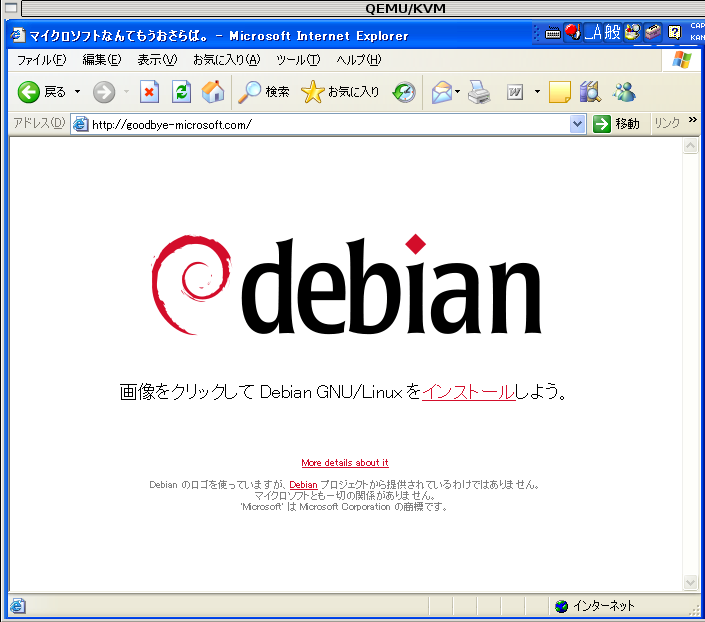
\includegraphics[width=6cm]{image200703/goodbyemicrosoftcom1.png}
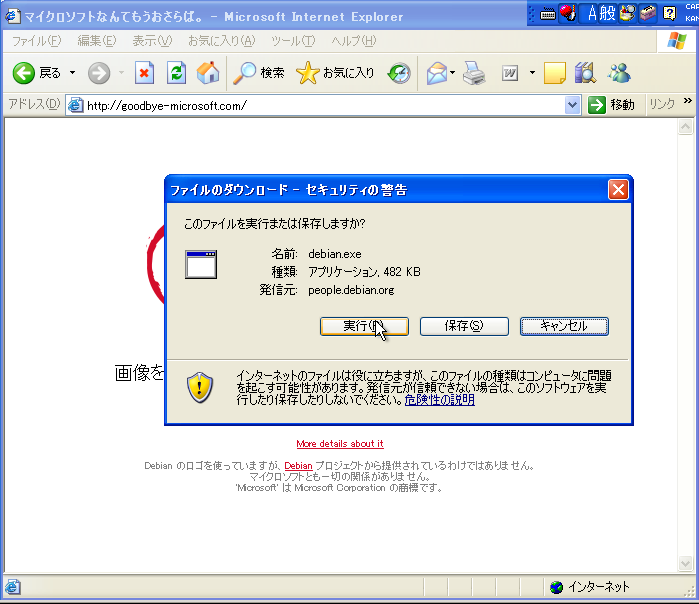
\includegraphics[width=6cm]{image200703/goodbyemicrosoftcom2.png}\\
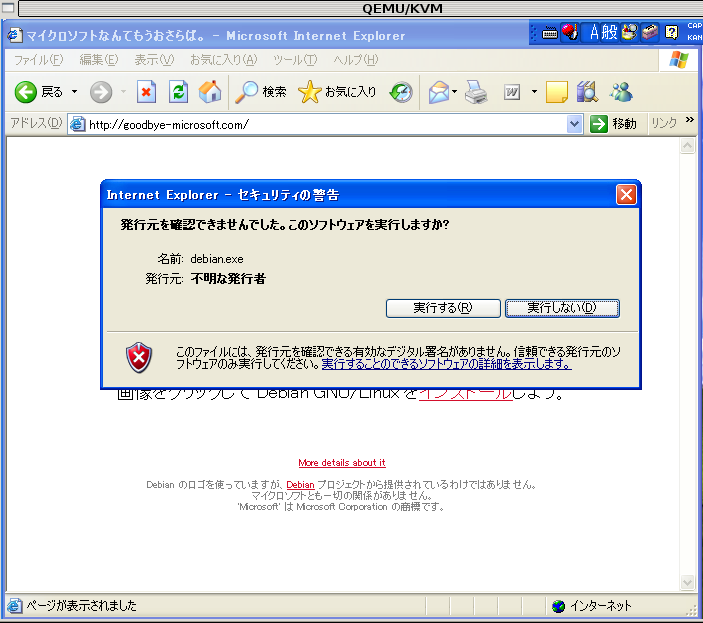
\includegraphics[width=6cm]{image200703/goodbyemicrosoftcom3.png}
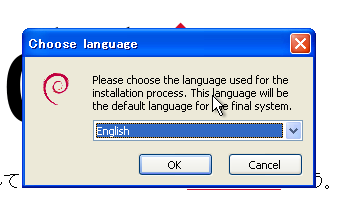
\includegraphics[width=6cm]{image200703/goodbyemicrosoftcom4.png}\\
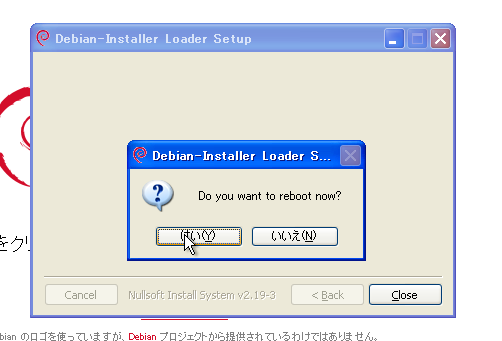
\includegraphics[width=6cm]{image200703/goodbyemicrosoftcom5.png}
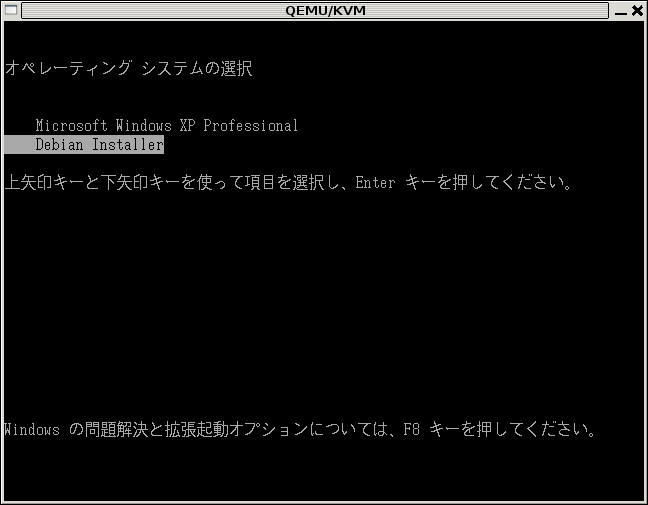
\includegraphics[width=6cm]{image200703/goodbyemicrosoftcom6.png}\\
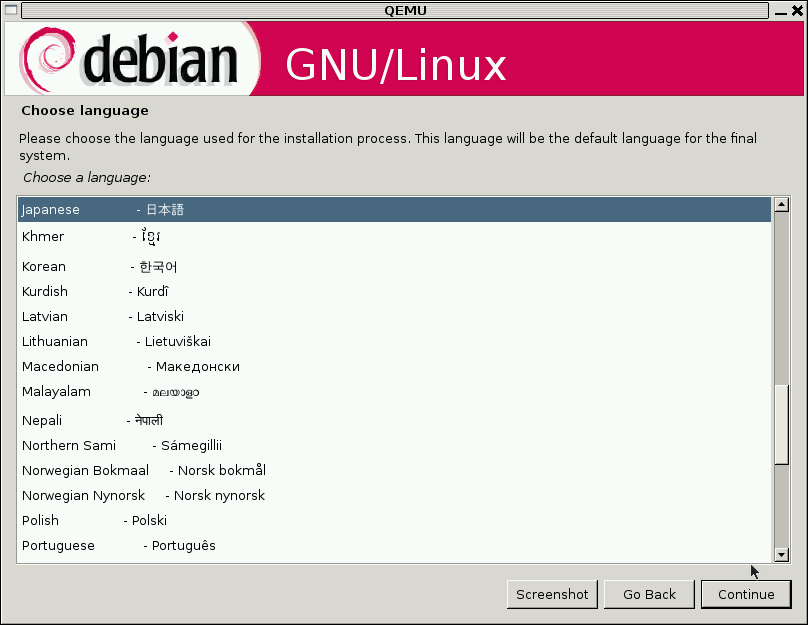
\includegraphics[width=6cm]{image200703/goodbyemicrosoftcom7.png}

\subsubsection{検証環境}

kvm を利用して、linux のインスタンスを起動して活用しています。

user-mode-linux と chroot を昔は使っていました。仮想環境を利用してくれる 
pbuilder-user-mode-linux というコマンドなどがあります。それを利用すると、
仮想環境の中でソフトウェアパッケージのビルドなどを行ってくれます。

\subsubsection{pasori}

USB 経由で接続する pasori というデバイスがあります。それを利用するために 
kvm を利用しています。EDY のチャージなどをする際に、Windowsのアプリケー
ションしかリリースされていないのですが、問題ありません。qemu (すなわち
kvm)には USB デバイスをゲストOSに直接見せる機能があります。それを利用す
ればゲストOSからデバイスが見えます。

\subsubsection{IE実行環境}

IE を利用する Windows 環境のために kvm を利用しています。
qemu の cow イメージの機能を使い、毎回使い捨てできる環境で利用しています。

%%% trivia quiz
\dancersection{仮想化友の会常識QUIZ}{上川 純一}

仮想化は最近流行しています。ただ、猫も杓子も仮想化といっている現状、本当
に常識をただしく理解してますか?
OSCの会場に到達できるみなさまであれば問題ないとは思いますが、念のため確
認テストをさせていただきます。

\subsection{仮想化の常識}

\santaku
{仮想化でのparavirtualization とはなにか}
{仮想用にOSが変更されている}
{パラパラで仮装する}
{並列で仮想化する}
{A}

\santaku
{Intel の VTって何?}
{「バレーボール取ってきて」}
{真空管(vacuum tube)}
{Intel社が提唱するCPUの仮想化支援の仕組}
{C}

\subsection{仮想化の利点}

\santaku
{Windows を仮想化環境で実行することによる利点は何か}
{Windows VISTA ではライセンスを考えくてすむようになる}
{Windows がフリーソフトウェアになる}
{Windows が Linux 上で動く}
{C}
% Windows VISTA の例

\subsection{仮想化の分類}

\santaku
{別途カーネルが独立して必要では無い仮想化実装はどれか}
{user-mode-linux}
{xen}
{openvz}
{C}

\santaku
{kvm はなぜカーネルのメインラインにマージされたか?}
{作者がイケメンだった}
{政治力}
{影響範囲のコードが小さい}
{C}

\santaku
{kvm は paravirtualization をどういう方式で実現しているか}
{仮想環境で実行されるLinuxカーネルが paravirt\underline{ }ops 機構を利用
し、VMCALL 命令を発行することでホストOSに連絡する}
{根性・気合い}
{愛情}
{A}

\subsection{仮想化の仕組の常識}

\santaku
{x86 CPU において VMEXIT を発行する命令として、代表例である CPUID 命令の OPCODEは下記のうちどれ
か。}
{0x55}
{0x0f 0xa2}
{0x5d}
{B}
% 55, 5d はそれぞれ push/pop ebx

\santaku
{AMD-VとIntel-VT の一番大きな違は次のどれか}
{会社が違う}
{命令が違う}
{思い入れが違う}
{A}

\santaku
{Xen の Domain-U の U は何か}
{Unprivileged}
{User}
{Unix}
{A}

\santaku
{Xen という名前は何から由来したか}
{Xeno}
{作者の娘の名前}
{禅寺}
{A}

\santaku
{KVMはなんの略か}
{Keyboard Video Mouse}
{Kernel-based Virtual Machine}
{「これ持ってる?」「こんなビデオ持ってるぜ」}
{B}

\santaku
{i386 の場合の Domain-U の ring level は何?}
{1}
{2}
{3}
{A}

\subsection{Debian での常識}

\santaku
{Debian Project で推奨する仮想化の技術は?}
{xen}
{kvm}
{DFSGに合致するものならなんでもよい}
{C}

\dancersection{Windows から使える Debian 技術}{山根}

\subsection{Windows で Debian}

(CoLinux/VMWare/etc)

\subsection{goodbye-microsoft.com}

\subsection{cygwin/debian?}



\dancersection{KVM: Debian の仮想化技術紹介}{前田さん}

\subsection{xen}
\subsection{user-mode-linux}
\subsection{openvz}



\subsection{linux-vserver}
\subsection{各種エミュレータ}

qemu(i386, arm, x86-64), aranym(m68k), hercules(s390) などが
Linux が動作するという観点からは実用レベル。

\subsection{kvmの使いかた紹介}

\subsubsection{インストール方法}

kernel 2.6.20 以上の場合\footnote{KVMのユーザ空間とカーネル空間のバージョ
ンの整合性の問題があるため、今後もこの操作がうまくいくとは限らない。}
\begin{commandline}
 apt-get install kvm
\end{commandline}

kernel 2.6.20 以前の場合
\begin{commandline}
 apt-get install kvm
 m-a a-i kvm
\end{commandline}

利用方法、
動作確認した内容など。

\subsubsection{開発検証用}

\subsubsection{セキュリティーサンドボックス}

\subsubsection{アプライアンス}
スナップショットから復旧

\subsubsection{kvm で windows}

\subsubsection{kvm で Edy チャージ}

USBを認識させればよいじゃん。必殺技。

\begin{commandline}
kvm -localtime -hda winxp.cow -m 400 -usb -usbdevice host:054c:01bb
\end{commandline}

\subsubsection{kvm で digress}

qemu を利用して d-i のデバッグを行う。

\subsubsection{kvm で Edy チャージ}


\subsection{仮想化の濃い話}
\subsubsection{仮想化を使って退社しました}
\subsubsection{正式にLinuxカーネルへ取り込まれた仮想化技術KVM(Kernel-based Virtual Machine)について解説する。}


超マニアックな解説予定。

\dancersection{最後に}{}

勉強会の URL を紹介する。

質問のある人は展示場に来てください。
答えますよ。

宣伝告知、勉強会やりますか。


\cleartooddpage

\begin{minipage}[b]{0.2\hsize}
 \definecolor{titleback}{gray}{0.9}
 \colorbox{titleback}{\rotatebox{90}{\fontsize{80}{80} {\gt デビアン勉強会} }}
\end{minipage}
\begin{minipage}[b]{0.8\hsize}

\vspace*{15cm}
\hrule
\vspace{2mm}

\includegraphics[width=2cm]{image200502/openlogo-nd.eps}
\noindent \Large \bf Debian 勉強会資料\\ \\
\noindent \normalfont \debmtgyear{}年\debmtgmonth{}月\debmtgdate{}日 \hspace{5mm}  初版第1刷発行\\
\noindent \normalfont 東京エリア Debian 勉強会 (編集・印刷・発行)\\
\hrule
\end{minipage}

\end{document}
